% Teilauswertung X

\section{Aufnahme der Sensitized Emission}

In diesem Teil der Auswertung sollen die Bilder der Sensitized Emission und der FRET-Effizienz bestimmt werden.

\subsection{Bestimmung der Korrekturfaktoren}

Zu aller erst ist es notwendig Korrekturfaktoren zu bestimmen, um sogenannte Crosstalk Verunreinigungen zu beheben. Eine genauere Erklärung was Crosstalk Verunreinigungen sind und warum sie existieren findet sich in Abschnitt \ref{sec:verunreinigung}. \\

Folgende Korrekturfaktoren werden benötigt: 
\begin{align}
    \label{eq:korfakA}
    \alpha = \frac{D_{YFP}}{A_{YFP}}\\
    \beta = \frac{S_{CFP}}{D_{CFP}}\\
    \gamma = \frac{S_{YFP}}{A_{YFP}}\\
    \delta = \frac{D_{YFP}}{s_{YFP}}
    \label{eq:korfakB}
\end{align}

Bedeutung der Formelsymbole: 
\begin{itemize}
    \item D: Mit Anregung und Detektion des Donors
    \item A: Mit Anregung und Detektion des Akzeptors
    \item S: Mit Anregung des Donors und Detektion des Akzeptors
\end{itemize}

Erklärung der Indizes:
\begin{itemize}
    \item CY: Probe enthält beide Farbstoffe
    \item YFP: Probe enthält nur YFP
    \item CFP: Probe enthält nur CFP
\end{itemize}

\newpage
Im Folgenden soll nun anhand eines Beispiels die Vorgehensweise demonstriert werden, mit der die jeweiligen Werte für die Korrekturfaktoren bestimmt werden.\\

Als Beispiels haben wir den Wert $D_{YFP}$ ausgewählt.\\
Zuerst wird ein Bild einer Probe aufgenommen, welches die passenden Farbstoffe enthält (hier nur YFP). Außerdem wird der passende Aufnahmemodus gewählt, hier Anregung und Detektion des Donors.\\
Danach werden in diesen mithilfe der Programms Fiji die Mittelwerte bestimmter ROI's (Region of interest) bestimmt. Eine ROI wird in einem zellfreien Bereich platziert, um den Wert des Hintergrundes zu erfassen können ($D_{YFP(bg)}$). Die andere ROI wird um die Membran der Zelle gelegt ($D_{YFP(mb)}$). Dies wird in Abbildung \ref{fig:VerschROI} an einem Beispiel verdeutlicht.

\begin{figure}[h]
    \centering
    \begin{subfigure}[]{0.45\textwidth}
        \centering
        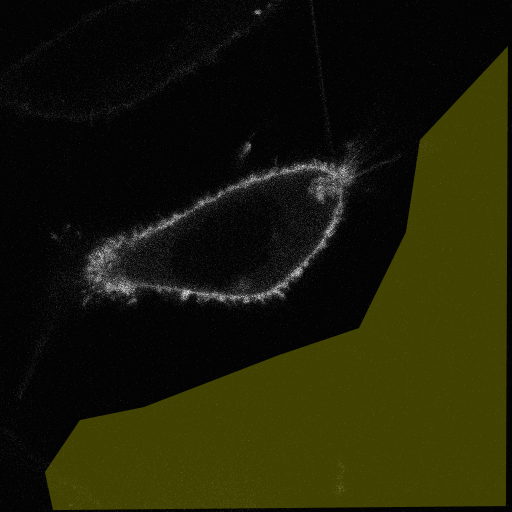
\includegraphics[width=\textwidth]{Paul/D-CY-bg.png}
        \caption{Beispiel: ROI des Hintergrundes}
    \end{subfigure}
    \hfill 
    \begin{subfigure}[]{0.45\textwidth}
        \centering
        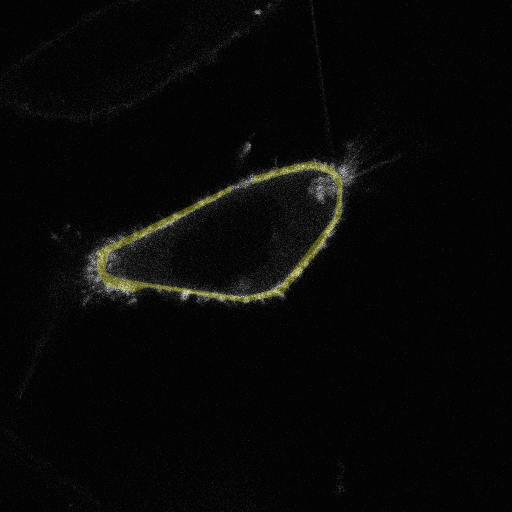
\includegraphics[width=\textwidth]{Paul/D-CY-zm.png}
        \caption{Beispiel: ROI der Zellmembran}
    \end{subfigure}
    \caption{Verschiedene ROI in $D_{CY}$ (hier: Zelle CY1)}
    \label{fig:VerschROI}
\end{figure}

Um nun der Wert zu bestimmen wird der Hintergrundwert abgezogen: 
\begin{align}
    D_{YFP} = D_{YFP(mb)} - D_{YFP(bg)}
\end{align}

\newpage
Dieser Vorgang wurde in analoger Weise für alle anderen Werte wiederholt. Dannach werden die Gleichungen \ref{eq:korfakA} bis \ref{eq:korfakB} verwendet um die Korrekturfaktoren zu berechnen. Dabei haben sich folgende Werte ergeben: \\

\begin{table}[h]
    \centering
    \begin{tabular}{c|c|c|c}
         Messung Nr. &        $D_{CFP}$ &           $S_{CFP}$ &      $\beta$ \\ \hline\hline
               1 &  102.466 &      18,805 &  0.183524 \\\hline
               2 &   68.186 &      12,936 &  0.189716 \\\hline
               3 &   15.184 &       2,796 &  0.184141 \\\hline
               4 &   38.030 &       6,681 &  0.175677 \\\hline
               5 &   27.955 &        4,86 &  0.173851 \\\hline
               6 &   18.747 &       3,229 &  0.172241 \\\hline
               7 &   89.738 &      16,416 &  0.182933 \\\hline
               8 &   56.398 &      10,034 &  0.177914 \\\hline
               9 &   58.660 &      10,779 &  0.183754 \\\hline
              10 &   50.819 &       8,977 &  0.176647 \\\hline
        \end{tabular}
    \caption{Messungen für CFP markierte Zellen zur Bestimmung von $\beta$}
\end{table}

\begin{table}[h]
    \centering
    \begin{tabular}{c|c|c|c|c|c|c}
         Messung Nr. &  $D_{YFP}$ & $A_{YFP}$ & $S_{YFP}$ &     $\alpha$ &     $\gamma$ &     $\delta$ \\\hline\hline
         1 &  1.685 &  179.276 &  97.906 &  0.009399 &  0.546119 &  0.017210 \\\hline
         2 &  0.371 &   40.330 &  17.076 &  0.009199 &  0.423407 &  0.021726 \\\hline
         3 &  0.529 &   94.979 &  38.451 &  0.005570 &  0.404837 &  0.013758 \\\hline
         4 &  0.538 &   60.703 &  25.409 &  0.008863 &  0.418579 &  0.021174 \\\hline
         5 &  0.429 &   75.727 &  32.435 &  0.005665 &  0.428315 &  0.013226 \\\hline
         6 &  0.533 &   63.920 &  27.325 &  0.008339 &  0.427487 &  0.019506 \\\hline
         7 &  0.651 &  114.199 &  48.084 &  0.005701 &  0.421054 &  0.013539 \\\hline
         8 &  0.490 &   31.834 &  13.232 &  0.015392 &  0.415656 &  0.037031 \\\hline
         9 &  0.598 &   80.300 &  34.689 &  0.007447 &  0.431993 &  0.017239 \\\hline
        10 &  0.607 &   72.924 &  30.036 &  0.008324 &  0.411881 &  0.020209 \\\hline
        \end{tabular}
    \caption{Messungen für YFP markierte Zellen zur Bestimmung von $\alpha$, $\gamma$ und $\delta$}
\end{table}

Somit ergeben sich folgende Mittelwerte für die Korrekturfaktoren: 
\begin{align}
    \alpha = (0,008 \pm 0,003)\\
    \beta = (0,180 \pm 0,006)\\
    \gamma = (0,43 \pm 0,04)\\
    \delta = (0,019 \pm 0,007)
\end{align}
Der Fehler wurde über die Standardabweichung berechnet.

\newpage
\subsection{Bestimmung der Sensitized Emission und FRET-Effizienz Bilder}

Mithilfe der Korrekturfaktoren können die Bilder der Sensitized Emission und der FRET-Effizienz, unter Verwendung folgender Formeln und des Programms Fiji, errechnet werden.
\begin{align}
    SE &= \frac{S_{CY} - \beta \cdot D_{CY} - (\gamma -\alpha \beta)\cdot A_{CY}}{1 - \beta \delta} \\
    E &= \frac{SE}{\sqrt{A_{CY} \cdot D_{CY}}}
\end{align}

Nachfolgend sind ausgewählte Bilder abgebildet die aus diesen Formeln resultieren.

\begin{figure}[h]
    \centering
    \begin{subfigure}[]{0.45\textwidth}
        \centering
        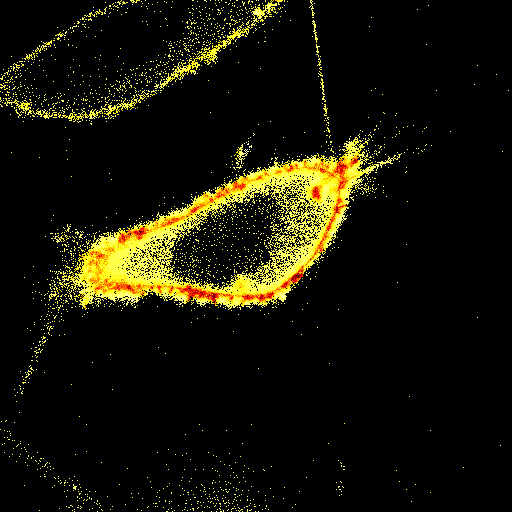
\includegraphics[width=\textwidth]{Paul/SE1.png}
        \caption{SE Bild der Aufnahme CY1}
    \end{subfigure}
    \hfill 
    \begin{subfigure}[]{0.45\textwidth}
        \centering
        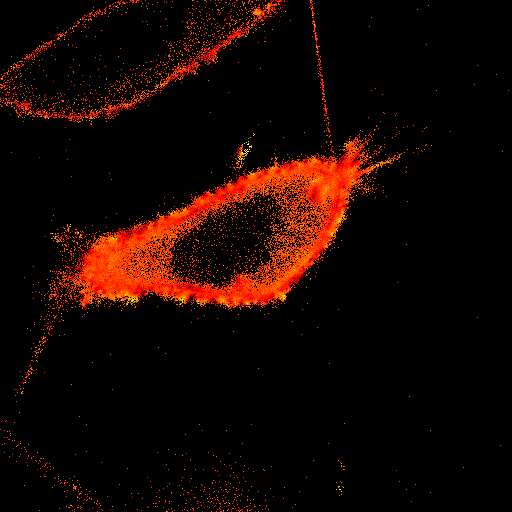
\includegraphics[width=\textwidth]{Paul/E1.png}
        \caption{E Bild der Aufnahme CY1}
    \end{subfigure}
    \caption{Zelle CY1 in SE und E}
\end{figure}

\begin{figure}[h]
    \centering
    \begin{subfigure}[]{0.45\textwidth}
        \centering
        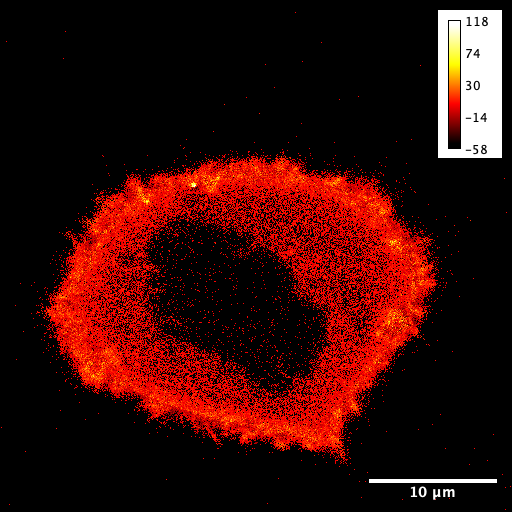
\includegraphics[width=\textwidth]{Paul/SE3.png}
        \caption{SE Bild der Aufnahme CY3}
    \end{subfigure}
    \hfill 
    \begin{subfigure}[]{0.45\textwidth}
        \centering
        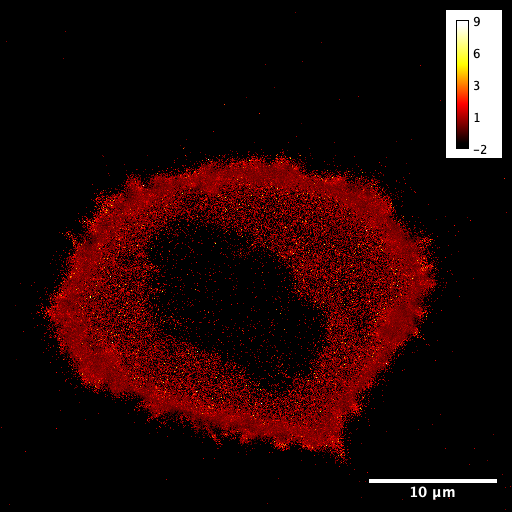
\includegraphics[width=\textwidth]{Paul/E3.png}
        \caption{E Bild der Aufnahme CY3}
    \end{subfigure}
    \caption{Zelle CY3 in SE und E}
\end{figure}

\newpage
\section{Donoremission nach Akzeptorbleichung}
